% Set up the document
\documentclass{article}

% Page size
\usepackage[
    letterpaper,]{geometry}

% Lines between paragraphs
\setlength{\parskip}{\baselineskip}
\setlength{\parindent}{0pt}

% Math
\usepackage{mathtools}
\usepackage{amssymb}
\usepackage{amsthm}
\usepackage{commath}

% Number sets
\newcommand{\C}{\mathbb{C}}
\newcommand{\N}{\mathbb{N}}
\newcommand{\Q}{\mathbb{Q}}
\newcommand{\R}{\mathbb{R}}
\newcommand{\Z}{\mathbb{Z}}

% Links
\usepackage{hyperref}

% Page numbers at top right
\usepackage{fancyhdr}
\pagestyle{fancy}
\fancyhf{}
\fancyhead[R]{\thepage}
\renewcommand\headrulewidth{0pt}

% Graphics
\usepackage{float}
\usepackage{graphicx}
\graphicspath{ {./img/} }

\begin{document}

\textbf{MATH 461 assignment 4} \\
\textbf{Matt Wiens \#301294492} \\
\textbf{2020-07-03}

3.9.2. Psychologists interested in learning theory study learning
curves. A learning curve is a graph of a function $P(t)$, the
performance of someone learning a skill as a function of the training
time $t$.

(a) What does $\od{P}{t}$ represent?

\textit{Solution.}
The derivative $\od{P}{t}$ represents the rate at which an individual is
learning at time $t$ into their training time.

\vspace{5mm}

(b) Discuss why the differential equation
%
\begin{equation*}
    \dod{P}{t} = k (M - P),
\end{equation*}
%
where $k$ and $M$ are positive constants, is a reasonable model for
learning. What is the meaning of $k$ and $M$? What would be a reasonable
initial condition for the model? Include a graph of $\od{P}{t}$ versus
$P$ as part of your discussion.

\textit{Solution.}
Qualitatively, for $P \leq M$ the $M - P$ term says that the rate at
which you learn decreases the more you learn (i.e., the better your
performance), up to some maximum performance level $M$, after which you
stop learning. This is fairly intuitive for me.

For $P > M$, this term says that your performance will decay down to $M$
at a rate proportional to the difference between your performance and the
``maximum'' performance level. I find this case quite a bit less intuitive
than $P \leq M$, but it is a reasonable assumption that $P \leq M$ whenever
this is applied, allowing us to ignore this case.

The constant $k$ essentially scales the $M - P$ term, and so governs how
rapidly one learns (or decays for $P > M$) at any given performance level $P$.

Based on my comments so far, I would say that any initial condition
with $P \leq M$ is reasonable for this model. $P > M$ could work too,
with proper justification in the particular application of this model.

A plot of the differential equation is shown, with the particular case
of $k = 1/3$, $M = 100$, in Figure~\ref{fig:q392a}.

\begin{figure}[!ht]
    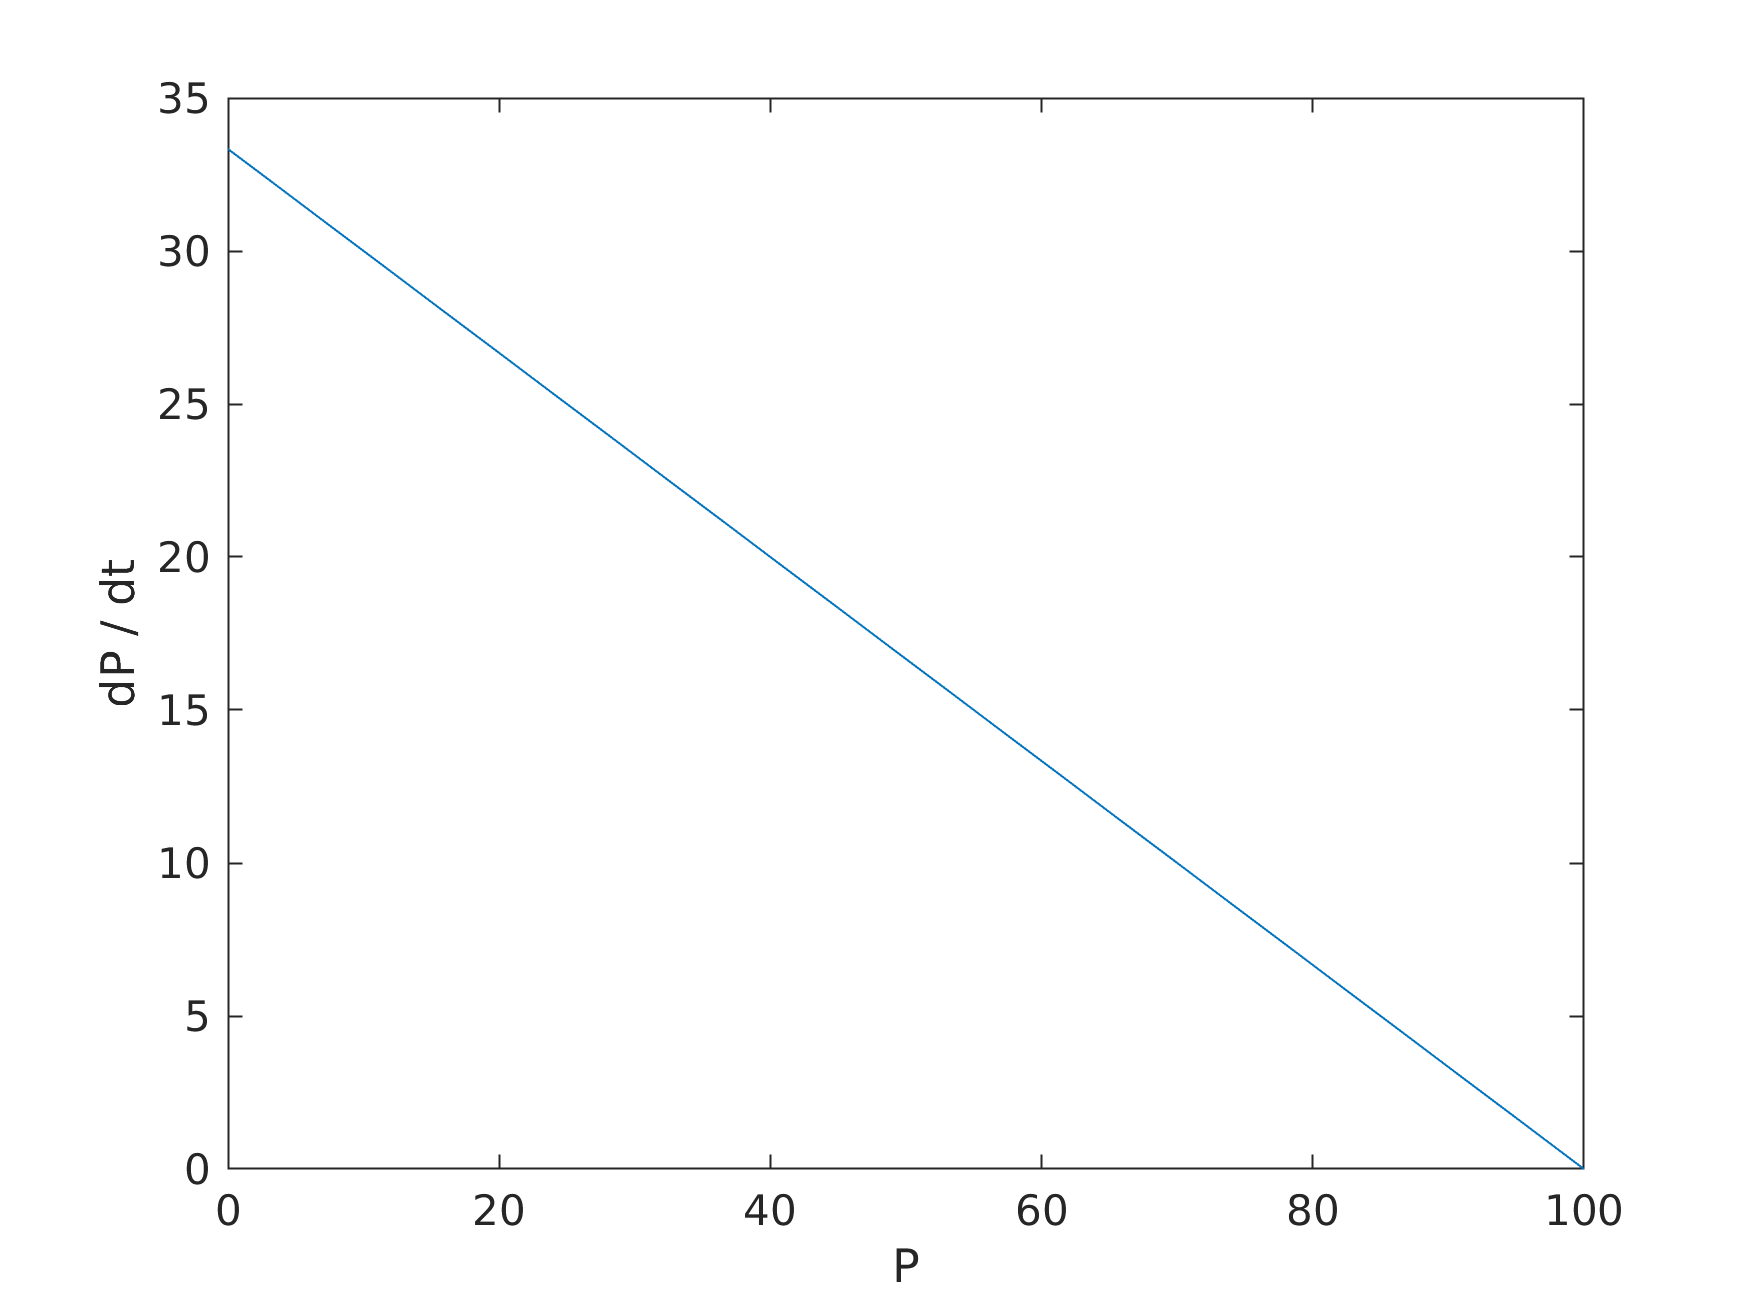
\includegraphics[width=5in]{q392a}
    \centering
    \caption{Plot of $\od{P}{t}$ versus $P$ for $k = 1/3$, $M = 100$}
    \label{fig:q392a}
\end{figure}

\vspace{5mm}

(c) Make a qualitative sketch of solutions to the differential equation.

\textit{Solution.}
Noting that
%
\begin{equation*}
    \dod{(M - P)}{t} = - \dod{P}{t} = - k (M - P)
\end{equation*}
%
we see that the change in learning decays down to zero exponentially in time.
This gives us enough to qualitatively sketch the solutions. However,
solving this system is very easy, so I'm going to go ahead and do it.
That is, the solutions are of the form
%
\begin{equation*}
    M - P = c e^{-k t} \implies P = M - c e^{-k t},
\end{equation*}
%
where the $c$ is related to the initial performance $P_0$ by
$c = M - P_0$. Hence our solutions are given by
%
\begin{equation*}
    P = M - (M - P_0) e^{-k t}
    .
\end{equation*}
%
The solution is plotted below in Figure~\ref{fig:q392b}, taking
different values of $k$ and fixing $P_0 = 0$, $M = 100$. (Varying $P_0$
isn't very insightful since this just amounts to horizontally
translating the solution curves.)

\begin{figure}
    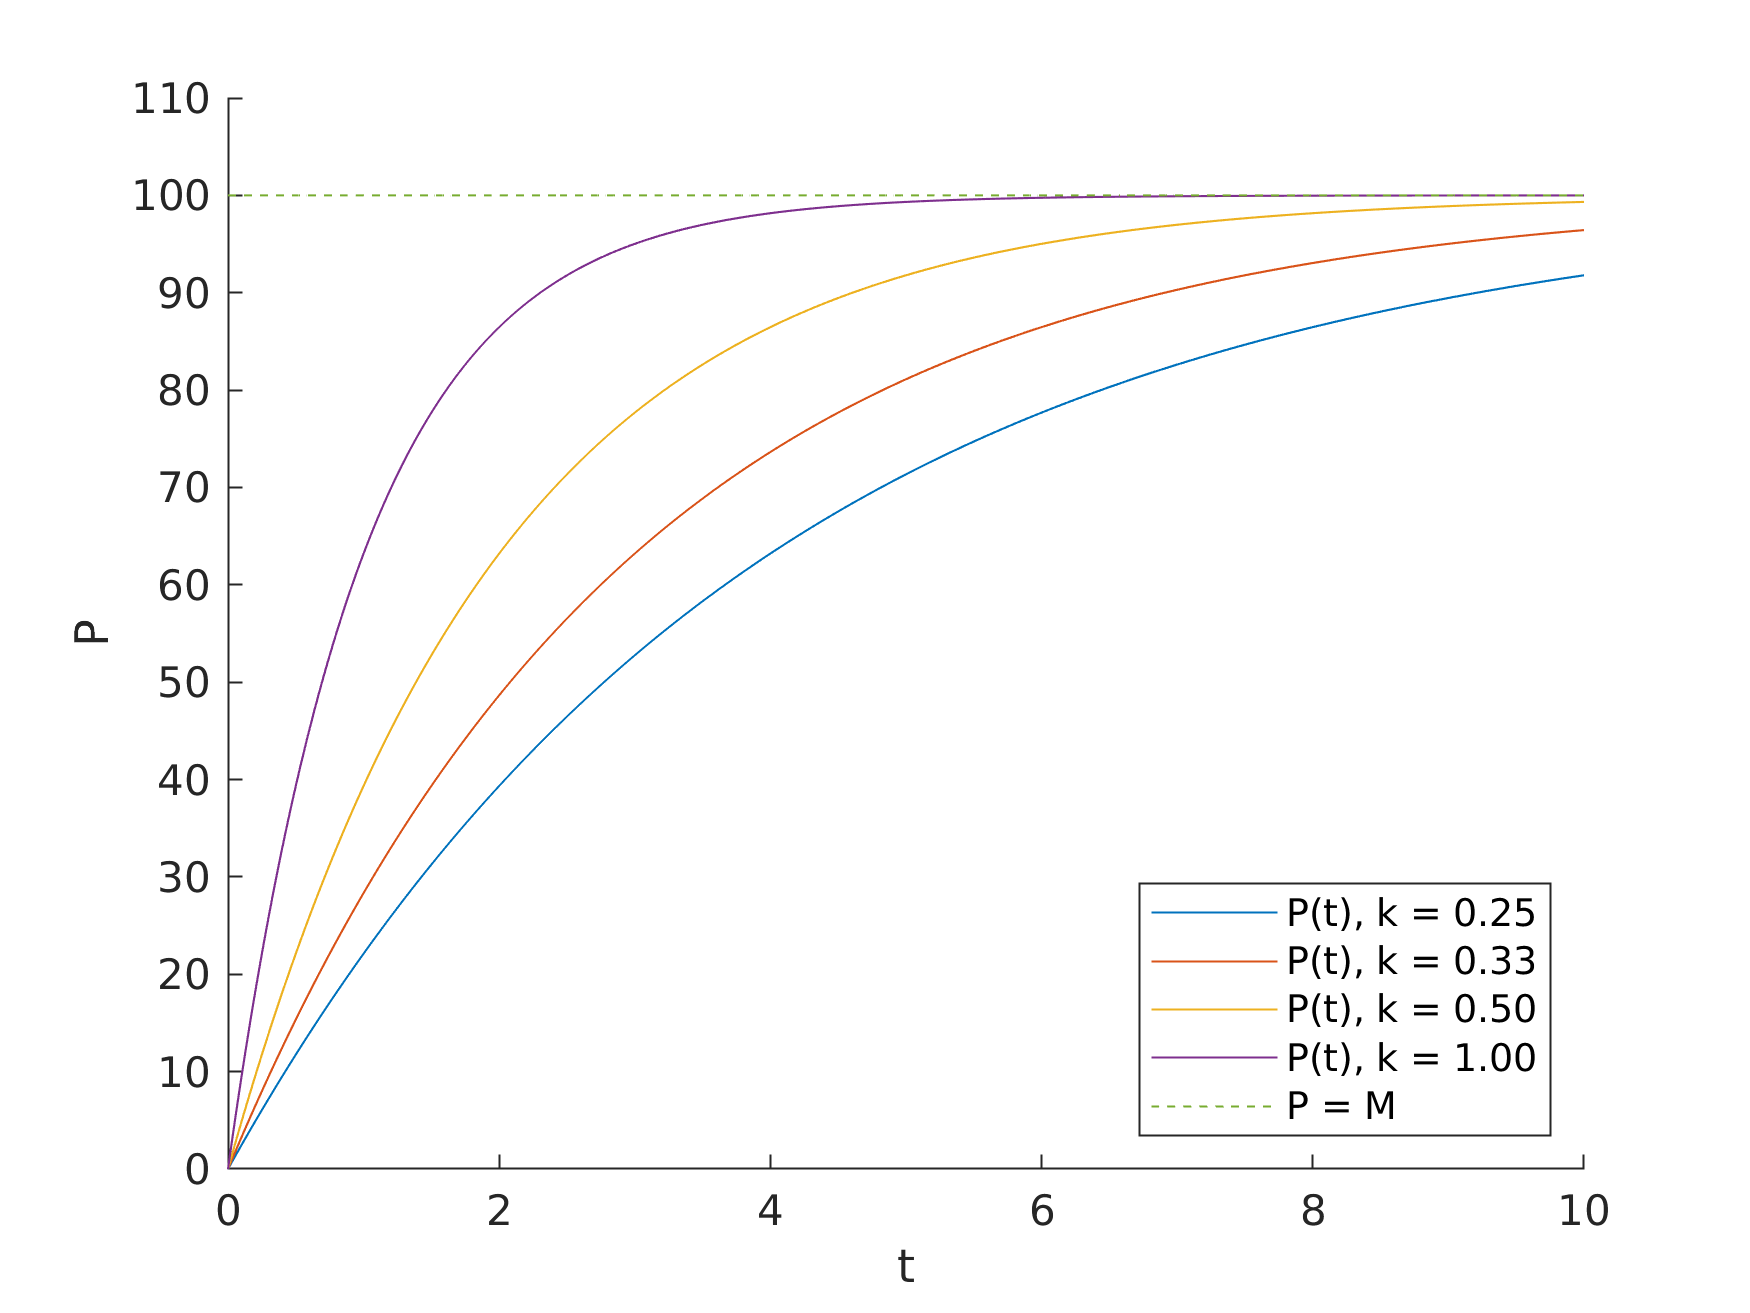
\includegraphics[width=5in]{q392b}
    \centering
    \caption{Plots of $P(t)$ for $P_0 = 0$, $M = 100$}
    \label{fig:q392b}
\end{figure}

\newpage

3.9.16. Some populations produce waste products, which in high concentrations are
toxic to the population itself. For example, algae or bacteria show the structure
in Figure 3.25 (in the course textbook). Let the population density be denoted
by $n(t)$ and the toxin concentration by $y(t)$. Then
%
\begin{align*}
    \dot{n} &= (\alpha - \beta - K y) n, \\
    \dot{y} &= \gamma n - \delta y,
\end{align*}
%
with $\alpha, \beta, \gamma, \delta, K \geq 0$.

(b) Find the nullclines and the steady states.

\textit{Solution.}
Following the notation in the textbook, let
%
\begin{align*}
    f_1(n, y) &= (\alpha - \beta - K y) n, \\
    f_2(n, y) &= \gamma n - \delta y
    .
\end{align*}
%
The $n$-nullcline is then the set of all points $(n, y)$ such that
$f_1(n, y) = 0$, which we can see by inspection is given by
%
\begin{equation*}
    \cbr{(0, y): y \geq 0} \cup \cbr{\del{n, \frac{\alpha - \beta}{K}}: n \geq 0}
    .
\end{equation*}
%
The $y$-nullcline, on the other hand, is the set of all points $(n, y)$
such that $f_2(n, y) = 0$. This is given by (again by inspection)
%
\begin{equation*}
    \cbr{\del{\frac{\delta y}{\gamma}, y}: y \geq 0}
    .
\end{equation*}
%
We can find the steady states by taking the intersection of the $n$- and
$y$-nullclines, but this system has so many parameters that its easier
just to use Maple to solve
%
\begin{align*}
    0 &= (\alpha - \beta - K y) n, \\
    0 &= \gamma n - \delta y.
\end{align*}
%
Solving the above system of equations in Maple we obtain the steady state
solutions
%
\begin{equation*}
    (n, y) \in \cbr{
        (0, 0),
        \del{
            \frac{\delta (\alpha - \beta)}{\gamma K},
            \frac{\alpha - \beta}{K}
        }}
        .
\end{equation*}

\vspace{5mm}

(d) Linearize the system and characterize each of the steady states
(stable/unstable, saddle, node, spiral, center, etc.). Find the regions
in parameter space such that the nontrivial (coexistence) equilibrium is
either a node or a spiral.

\textit{Solution.}
We start by computing the Jacobian matrix for our system:
%
\begin{equation*}
    J =
    \begin{bmatrix}
        \partial_n f_1 & \partial_y f_1 \\
        \partial_n f_2 & \partial_y f_2
    \end{bmatrix}
    =
    \begin{bmatrix}
        \alpha - \beta - K y & - K n \\
        \gamma & - \delta
    \end{bmatrix}
\end{equation*}
%
Evaluating this matrix at each of our steady states we have
(letting $J(n, y)$ denote the Jacobian evaluated at the point
$(n, y)$)
%
\begin{align*}
    J(0, 0) &=
    \begin{bmatrix}
        \alpha - \beta & 0 \\
        \gamma & - \delta
    \end{bmatrix}
    \eqqcolon J_0
    ,
    \\
    J \del{
            \frac{\delta (\alpha - \beta)}{\gamma K},
            \frac{\alpha - \beta}{K}
        }
    &=
    \begin{bmatrix}
        0 & - \frac{\delta (\alpha - \beta)}{\gamma} \\
        \gamma & - \delta
    \end{bmatrix}
    \eqqcolon J_1
    .
\end{align*}
%
For $J_0$ we can see that the eigenvalues are simply the diagonal elements,
that is $\lambda_1 = \alpha - \beta$, $\lambda_2 = - \delta$. Since we
know that $\delta \geq 0$, either $(0, 0)$ is a saddle or an unstable node,
depending on whether $\lambda_1 < 0$ or not, respectively.

For $J_1$ we compute the characteristic polynomial and set it to zero:
%
\begin{equation*}
    \det(J_1 - \lambda I) = \lambda^2 + \delta \lambda + \delta (\alpha - \beta) = 0
    .
\end{equation*}
%
This has solutions
%
\begin{equation*}
    \lambda = - \frac{\delta}{2} \pm \frac{1}{2} \sqrt{\delta^2 - 4(\alpha - \beta)}
    .
\end{equation*}
%
This will be a node provided that
%
\begin{equation*}
    \delta^2 \geq 4 (\alpha - \beta)
\end{equation*}
%
(note that both eigenvalues will be real and negative in this case); otherwise
the coexistence equilibrium will be a stable spiral.

\vspace{5mm}

(e) Sketch some trajectories for the case of $\delta < 4(\alpha - \beta)$,
and explain what you see in terms of the biology.

\textit{Solution.}
do this tomorrow

\newpage

3.9.17. Imagine a small pond that is mature enough to support wildlife.
We desire to stock the pond with game fish, say trout or bass. Let $T(t)$
denote the population of the trout at any time $t$, and let $B(t)$
denote the bass population.

(a) Initially, assume that the pond environment can support an unlimited
number of trout in isolation (i.e., growth of the trout population is
exponential). Write down an equation that describes the evolution of the
trout population in the absence of competition.

\textit{Solution.}
In this case the 

\vspace{5mm}

(b) Modify the equation to account for competition of the trout with the
bass population for living space and a common food supply. You may assume
that the growth rate of the trout population depends linearly on the bass
population.

\textit{Solution.}

\vspace{5mm}

(c) Repeat (a) and (b) for the bass population.

\textit{Solution.}

\vspace{5mm}

(e) What are the steady states of the system? Determine stability of the
steady states using linearization.

\textit{Solution.}

\end{document}
